\documentclass[conference]{IEEEtran}
\IEEEoverridecommandlockouts
% The preceding line is only needed to identify funding in the first footnote. If that is unneeded, please comment it out.
\usepackage{cite}
\usepackage{amsmath,amssymb,amsfonts}
\usepackage{algorithmic}
\usepackage{graphicx}
\usepackage{textcomp}
\usepackage{xcolor}
\usepackage{physics}
\usepackage{hyperref}
\def\BibTeX{{\rm B\kern-.05em{\sc i\kern-.025em b}\kern-.08em
    T\kern-.1667em\lower.7ex\hbox{E}\kern-.125emX}}
\begin{document}

\title{RAID-6 Based Distributed Storage System}

\author{
\IEEEauthorblockN{Liu Yihao}

\IEEEauthorblockA{\small\textit{School of Computer Science and Engineering} \\
\textit{Nanyang Technological University}\\
Singapore \\
yihao002@e.ntu.edu.sg}
\and
\IEEEauthorblockN{Liu Ruicheng}
\IEEEauthorblockA{\small\textit{School of Computer Science and Engineering} \\
\textit{Nanyang Technological University}\\
Singapore \\
ruicheng001@e.ntu.edu.sg}
\and
\IEEEauthorblockN{Tang Bin}
\IEEEauthorblockA{\small\textit{School of Computer Science and Engineering} \\
\textit{Nanyang Technological University}\\
Singapore \\
tang0458@e.ntu.edu.sg}
}

\maketitle

\begin{abstract}
We implemented a RAID-6 based distributed storage system in order to achieve fault tolerance as well as efficient communication among data nodes. We employed Reed-Solomon Code in file encoding and decoding and a peer-to-peer reliable array of independent nodes network to carry out communication between different data nodes. The experiment result shows that our system is robust and adaptive while retaining a reasonable time complexity.
\end{abstract}

\begin{IEEEkeywords}
RAID-6, RAIN, Reed Solomon Codes, peer-to-peer, distributed system
\end{IEEEkeywords}

\section{Introduction}

\subsection{Objectives}\label{sec:intro}

In this project, we designed and implemented a RAID-6 based distributed storage system. The system have following functionalities:

\begin{itemize}
    \item Store Data objects in data nodes using (generalized) RAID-6 for fault-tolerance.
    \item Detect failure of storage nodes.
    \item Rebuild of lost redundancy at a replacement storage node.
    \item Support arbitrary size of data objects.
    \item Deploy the system across multiple containers to realize a peer-to-peer RAIN.
    \item Support mutable files, with CRUD operations and considering consistency issues.
    \item Support larger set of configurations, including up to 255 primary and parity nodes.
    \item Optimize the encoding and decoding matrix operations on finite field.
\end{itemize}

\subsection{RAID}

Reduce data lost and ensure fast data retrieval are two important aspects of data storage. Redundant Array of Independent Disk (RAID) is a way of storing data in multiple disks into a single array in order to protect data from disk failure and achieve great performance. 

RAID was introduced in 1988\cite{patterson1988case}. Instead of reading and writing from single, large and expensive high performing disk driver, RAID placing data on multiple independent and inexpensive disks and logically putting them together as an array which appear as a single logical drive to an operating system. These inexpensive disks working together archived speed and/or reliability of single expensive disk. However, the data exact speed and reliability depend on RAID version. 

RAID 0 employs striping which divide the write over multiple disks. When data striped across, it is split into chunks and each chunk is written to at least one of the underlying devices. This design has no redundancy of data which lead to no fault tolerance but it offers the best performance. 

RAID 1 also known as disk mirroring which at least two disk drives that duplicate the storage of data. In the event of either drive failure, data still available in another disk. RAID 1 has no striping so write operation is the same as single disk however the read operation improved due to the duplication. 

RAID 10 combining RAID 1 and RAID 0, the data is mirrored then the mirrors are striped. RAID 10 requires at least 4 drives which 2 mirrored drives hold half of the striped data and another 2 mirrored drives hold the rest. RAID 10 is able to afford to loss at most two disks. 

RAID 5\cite{chen1994raid} based on distributed parity and striping. Parity is a data integrity mechanism which used to reconstruct data if a disk fails and parity distributed across all available disks to ensure redundancy and performance. RAID 5 is able to afford at most 1 disk failure. 

RAID 6\cite{anvin2007mathematics} introduced a second parity on top of RAID 5 which is able to withstand two disks failure. Like other RAID version, RAID 6 strips data across multiple disks to increase performance, but the additional parity also lead to complex calculation to determine the parity data, hence RAID 6 has slower write performance than RAID 5.

In general, RAID 0 is good when performance is critical and data is not significantly important. RAID 1 provide an inexpensive way to gain additional data redundancy to ensure high up-time. RAID 5 and 6 are the most common configuration for business and enterprise since they provide better performance than mirroring as well as fault tolerance.

In this report, we first introduced various version of RAID, then presented some key concepts including Redundant Array of Independent Nodes and Reed-Solomon Codes. We implemented a distributed storage system based on RAID 6 using C++ and Python. Along with implementation, we described the system architecture, explained the implementation details and presented the experiments and findings. 

\subsection{Redundant Array of Independent Nodes}
RAIN\cite{rodriguez2006policy} (also called channel bonding, redundant array of independent nodes, reliable array of independent nodes, or random array of independent nodes) is a cluster of nodes connected in a network topology with multiple interfaces and redundant storage. RAIN is used to increase fault tolerance. It is an implementation of RAID across nodes instead of across disk arrays.

RAIN can provide fully automated data recovery in a local area network (LAN) or wide area network (WAN) even if multiple nodes fail. A browser-based, centralized, secure management interface facilitates monitoring and configuration from a single location. There is no limit to the number of nodes that can exist in a RAIN cluster. New nodes can be added, and maintenance conducted, without incurring network downtime.

RAIN originated in a research project for computing in outer space at the California Institute of Technology (Caltech), the Jet Propulsion Laboratory (JPL), and the Defense Advanced Research Projects Agency (DARPA) in the United States. The researchers were looking at distributed computing models for data storage that could be built using off-the-shelf components.

The idea for RAIN came from RAID (redundant array of independent disks) technology. RAID partitions data among a set of hard drives in a single system. RAIN partitions storage space across multiple nodes in a network. Partitioning of storage is called disk striping. Several patents have been granted for various proprietary versions of RAIN.

\subsection{Reed-Solomon Codes}
Reed-Solomon codes\cite{reed1960polynomial} are block-based error correcting codes with a wide range of applications in digital communications and storage. Reed-Solomon codes are used to correct errors in many systems including: Storage devices (including tape, Compact Disk, DVD, barcodes, etc); wireless or mobile communications (including cellular telephones, microwave links, etc); satellite communications; digital television or DVB and high-speed modems such as ADSL, xDSL, etc.

The Reed-Solomon encoder takes a block of digital data and adds extra "redundant" bits. Errors occur during transmission or storage for a number of reasons (for example noise or interference, scratches on a CD, etc). The Reed-Solomon decoder processes each block and attempts to correct errors and recover the original data. The number and type of errors that can be corrected depends on the characteristics of the Reed-Solomon code.

Reed Solomon codes are a subset of BCH codes and are linear block codes. A Reed-Solomon code is specified as $RS(n,k)$ with s-bit symbols.

This means that the encoder takes $k$ data symbols of $s$ bits each and adds parity symbols to make an $n$ symbol codeword. There are $n-k$ parity symbols of $s$ bits each. A Reed-Solomon decoder can correct up to $t$ symbols that contain errors in a codeword, where $2t = n-k$.

Reed-Solomon encoding and decoding can be carried out in software or in special-purpose hardware. Reed-Solomon codes are based on a specialist area of mathematics known as Galois fields or finite fields. A finite field has the property that arithmetic operations (+,-,x,/ etc.) on field elements always have a result in the field. A Reed-Solomon encoder or decoder needs to carry out these arithmetic operations. These operations require special hardware or software functions to implement.


\section{System Architecture}

\subsection{File Encoding and Decoding}

We use MDS (``Maximum Distance Separable'') erasure coding to encode and decode the file objects. Suppose there are $k$ primary data strips and $m$ parity data strips, where $k\geqslant 1$ and $m\geqslant 0$, which sums up to $n$ data strips stored on $n$ data nodes in total. 

When a data nodes fails, the file objects stored on it will become unusable,
and the storage system detects this. This failure node is called an erasure. An MDS code can reconstruct the data from any $m$ failures. 

We use Reed-Solomon Code in the finite field $GF(2^w)$ as the MDS code. $w$ is usually fixed to 8 because the minimal data unit is byte (8 bits) on most operation systems. This will lead to a constraint $n\leqslant 2^w$ so that there will be at most 256 nodes in the system. If more data nodes are needed, the system can be extended by building it with a larger $w$, while $w=8$ is already enough for our project. 

We also support file objects of arbitrary size. Suppose a file object $F$ with $r$ bytes, first we add $p$ padding zeros to $F$ and form $F'$ so that $r'=r+p$ and $r' \equiv 0 \mod k$. Now the length of $F'$ is aligned to the number of primary data strips so that we can transform it into a matrix $D$ of $k$ rows and $r'/k$ columns. 

Now we need to define a generator matrix $G$ for the Reed-Solomon Code, the size of the matrix should be $n times k$ so that we can use matrix multiplication of $G$ and $D$ to form an encoded matrix $E$. We have two requirements of the generator matrix:
\begin{itemize}
    \item \textbf{Original data are stored in the primary data nodes.} The first $k$ rows of $G$ should be an identify matrix of order $k$, so that the first $k$ rows of $E$ is equal to $D$. This is also called \textit{systematic coding}\cite{ph:13:tut}.
    \item \textbf{Any $k$ data nodes can be used to decode the data.} A sub matrix $G'$ formed by any $k$ rows of $G$ should be invertible, so that we can decode by a sub matrix $E'$ formed by the corresponding $k$ rows of $E$, by matrix multiplication of $G'^{-1}$ and $E'$.
\end{itemize}

In summary, the encoding process can be described by
\begin{equation}
    E = GD.
\end{equation}

And the decoding process can be described by
\begin{equation}
    D = G'^{-1}E',
\end{equation}
where $G'$ and $E'$ are constructed by any same $k$ rows of $G$ and $E$. We also store the length of the original file object $F$ so that $D$ can be trimmed to its original length after it is decoded.  

A Cauchy generator matrix can be used to satisfy these requirements. The first $k$ rows is an identify matrix of order $k$, then the next $m$ rows can be generated by
\begin{equation}
    g_{ij} = 1 / (x_i + y_j) \text{ in } GF(2^w),
\end{equation}
where $x_i\in\{1,2,\cdots,m\}$, $y_j\in\{m+1,m+2,\cdots,n\}$.

It is proved that any sub matrix of a Cauchy generator matrix can be inverted in $GF(2^w)$\cite{roth1989mds}. We applied LU-factorization and Gaussian Elimination to solve the matrix inversion problem, which can be done in time complexity of $\order{k^3}$.

\subsection{Data Node}

There are two possible setups of data nodes. In our implementation, both setups are allowed by configuration.
\begin{itemize}
    \item The first is to distribute all primary data strips on $k$ data nodes, and all parity data strips on $m$ data nodes. The drawback of this method is that the network flow of the primary data nodes will be much higher than parity data nodes because usually a user only need to get the data on primary data nodes.
    \item The second is to distribute data strips randomly on all $n$ data nodes, which will lead to a balanced network flow and computing resource. The drawback of this method is that a user also need to retrieve random data strips so that the decoding process may consume more time.
\end{itemize}

Each data node runs a service, which saves one data strip of each file object on its local filesystem. The data strip contains the encoded binary data, and also some other useful information:
\begin{itemize}
    \item The parameters $k$, $m$, $n$ for pre-validation
    \item The total size of the file object
    \item The size of the data strip
    \item Path of the file object
    \item ID (row number in $E$) of the data strip
    \item Timestamp of the encoding time, for consistency
    \item Checksum of the file object, for final validation
\end{itemize}

In order to resolve consistency issue, we use file path to uniquely identify the file objects, and decide which data strip should be preserved by timestamp of a global clock. More specifically, if there are two data strips with the same path on a file node, we only preserve the one with the latest timestamp; if the timestamps are the same, we will preserve the newly received one.

\subsection{P2P RAIN Network}

Different data nodes can communicate with each other with a protocol. Since our system is a peer-to-peer network, the service on each data node is exactly the same, which covers the following functionalities:

\begin{itemize}
    \item \textbf{read file object}: accepts a string which indicates the path of the file, sends \textbf{read data strip} requests to other data nodes, and then decodes the received data strips into a file object. If the decoding is unsuccessful (number of received data strips is not enough, or file checksum mismatch), it will throw an error.
    \item \textbf{write file object}: accepts a string which indicates the path of the file and a file object in binary form, encodes the file object, and then sends \textbf{write data strip} requests to other data nodes.
    \item \textbf{delete file object}: accepts a string which indicates the path of the file, sends \textbf{delete data strip} requests to other data nodes.
    \item \textbf{read data strip}: accepts a string which indicates the path of the file, finds the data strip by the path on local filesystem and returns it, or throws an error if data strip not found.
    \item \textbf{write data strip}: accepts a string which indicates the path of the file and a data strip in binary form and saves the data strip on local filesystem.
    \item \textbf{delete file object}: accepts a string which indicates the path of the file, deletes the corresponding data strip on local filesystem.
\end{itemize}

Based on these functionalities, it's convenient to implement other CRUD (create, read, update, delete) client service.

\section{Implementation Details}

The project source code can be found on GitHub: \url{https://github.com/tc-imba/CE7490-Project2}.

\subsection{File Encoding and Decoding}

We tried some erasure coding library such as \textit{pyfinite}\cite{Emin2018pyfinite} but we found that the efficiency of those libraries did not achieve our expectation. We noticed that some other erasure coding library are implemented in C++ and are much more faster than the Python libraries. So we re-implemented all of the low-level algorithms (including operations on finite fields, matrix operations, encoding and decoding) ourselves with C++.  

All of this part is implemented in standard C++, which can be found in the \texttt{cpp} directory. We use \textit{cython}\cite{Robert2020Cython} to compile the C++ code into a library which can be directly used in Python, since we're using Python elsewhere the system.  

In the file \texttt{cpp/LUT.h}, we generated two LUTs (lookup tables) for the multiplication and division operations. Each table is an two-dimensional array with $256\times 256$ bytes. We used lookup tables because it can provide extremely fast $\order{1}$ operations on the finite field $GF(2^8)$, and the size of a table (65536 bytes) is considerably small.  

In the file \texttt{cpp/GF8.h}, we implemented two classes, \texttt{GF8} and \texttt{GF8Matrix}. The \texttt{GF8} class overloads all operations (addition, subtraction, multiplication and division) on the finite field $GF(2^8)$. The \texttt{GF8Matrix} implements matrix operations such as matrix multiplication and inversion on $GF(2^8)$ to help the encoding and decoding procedure. 

In the file \texttt{cpp/RSCode.h} and \texttt{cpp/RSCode.cpp}, we implemented the Reed-Solomon Codes. The parameters $k$, $m$, $n$ can be used to initialize an \texttt{RSCode} class, the the class instance supports two operations: encoding and decoding. 

All of the C++ code are carefully optimized for the project. For example, in the decoding process, we can skip some calculations if a data strip is a primary data strip. We will show the performance of our coding library in the experiment section.

\subsection{Data Node}

We studied that low-level communication protocols such as TCP and UDP may provide a best communication channel between servers. However, considering that the CPU-bound encoding and decoding algorithms are already implemented in C++, the rest of the system is IO-bound and can be handled by asynchronous web servers, which leads to a more user-friendly and readable implementation. 

We chose the \textit{fastapi}\cite{Sebastian2020fastapi} framework in Python to implement the web service. It is an asynchronous API (Application Programming Interface) framework which can handle high concurrency requests. Our six functionalities of the service can be transformed into six APIs:

\begin{itemize}
    \item \textbf{GET /read/filepath} implements \textbf{read file object}
    \item \textbf{POST /write/filepath} implements \textbf{write file object}
    \item \textbf{GET /delete/filepath} implements \textbf{delete file object}
    \item \textbf{GET /readblock/filepath} implements \textbf{read data strip}
    \item \textbf{POST /writeblock/filepath} implements \textbf{write data strip}
    \item \textbf{GET /deleteblock/filepath} implements \textbf{delete data strip}
\end{itemize}

In order to resolve consistency issues, we added a mutex lock for \textbf{POST /write/filepath} and \textbf{GET /delete/filepath} so that only one operation of the same path can be executed at the same time. Similarly, we also add another mutex lock for \textbf{POST /writeblock/filepath} and \textbf{GET /deleteblock/filepath}. 

The web service can be started with various command line options for flexibility of configurations:

\begin{verbatim}
  -h, --host TEXT          
        Host address
  -p, --base-port INTEGER  
        Port of the first server
  -d, --debug              
        Enable debug mode
  -s, --server-id INTEGER [required]
        ID of the current server 
  -k, --primary INTEGER    
        Number of primary data strips
  -m, --parity INTEGER     
        Number of parity data strips
  -r, --random             
        Enable random distribution
  --data-dir TEXT          
        Location of data strips
  --help                   
        Show this message and exit
\end{verbatim}

The \textit{fastapi} framework can also automatically generate a documentation for all those APIs on the path \textbf{/docs}. 


\subsection{P2P RAIN Network}

We use \textit{Docker} to deploy our services in containers. A container is similar to a virtual machine, but only user spaces in the containers on a same host system is separated, while the kernel space is shared. A container is generally more efficient than a virtual machine, and since we don't need to care about security issues in the project, it is the best choice of our deployment. 

We wrote a \texttt{Dockerfile} to compile the whole project into a Docker image, and than we can deploy the image into containers with different parameters for the experiments. Each container can only communicate with other containers through the web APIs, so it perfectly simulates a P2P RAIN Network on different servers. 

Users can send API requests to any of the living data nodes and get the same file object with a path. We also designed a dynamic redundancy rebuilding mechanism in this procedure. When a user sends \textbf{GET /read/filepath} to a data node, it will send  \textbf{GET /readblock/filepath} reuqests to all other data nodes. The data node will try to decode the received data, and if the decoding is successful (only $k$ valid data strips is necessary) and some of data nodes failed to return a valid data strip, we can induce that the redundancy is broken on these failing data nodes. Then we can make \textbf{POST /writeblock/filepath} requests to these failing data nodes and rebuild the redundancy dynamically.  

However, the dynamic redundancy rebuilding mechanism is not perfect. Some files may not be acquired by the users very often, which leads to a less chance that it would be rebuilt on the failure nodes. We also introduce a static redundancy rebuilding mechanism. When a data node detected that any other data node failed for $K$ times, a message will be sent to a central server which handles the whole network. Note that our network is a P2P network, so the central server only acts as a watchdog of the failures detected. It may suggest a data node to help rebuild all data objects on a replaced data node, but does not have the privilege to force the data node to do so. We implemented an API \textbf{GET /rebuild} on the data nodes to achieve this.

\subsection{Shortages}

In our implementation, we assumed that the port of the web services are continuous for ease of experiment. If we need to deploy the services on different physical servers with different host addresses, we need to let each server know the address and port of all other servers by a configuration file or dynamical detection. Another solution is to setup a proxy backend server such as \textit{nginx} to forward the requests.  

For consistency issues, we used a global clock instead of a event triggered clock such as a vector clock. This may lead to inconsistency due to the error of system clock on different data nodes. For more robust consistency, we should change the global clock implementation to a vector clock implementation in the future. 

We didn't use multi-processing and GPU accelerated matrix operations which may further optimize the the encoding and decoding algorithm. Multi-processing can be used because the matrix multiplication in the encoding and decoding process can be run in parallel if the columns of the right matrix is split into many parts. GPU accelerated matrix operations is widely used in machine learning and some libraries can be reused to produce the operations on the finite field. 

In the last, we didn't implement user authentication in this project because it needs another distributed user privilege management system which is not the main focus of the project. User authentication can be simply integrated into the \textit{fastapi} framework with help of distributed databases such as \textit{mongodb} in real world applications. 

\section{Experiments}

All of the experiments are conducted on a desktop computer with a 24-core CPU @ 3.8 GHz and 32 GB memory. Only one CPU core is actually used because all of the programs are written in single-processing, and the memory must be sufficient for encoding and decoding large files. The plots are generated by \textit{matplotlib}\cite{Hunter:2007}.

\subsection{Performance of File Encoding and Decoding}

We tested the execution time encoding and decoding algorithms with two different implementations: our C++ based implementation and a Python based open-source implementation \textit{pyfinite}. We used three representative file sizes to test the implementations: 1KB, 1MB and 1GB. 

We also tested different number of data nodes, and select two representative number: 8 nodes and 128 nodes. For each number of data nodes ($n$), we chose different number of primary data nodes ($k$) to examine the performance. All of the decoding time are analysed based on the worse setup of data to be decoded. More specifically, we always use as many parity data strips as possible to find an upper bound of the time of the decoding process. In the setup of no parity data strips, we can observe a dramatic drop of encoding and decoding time because nothing needs to be calculated. 

\begin{figure}[htbp]
    \centering
    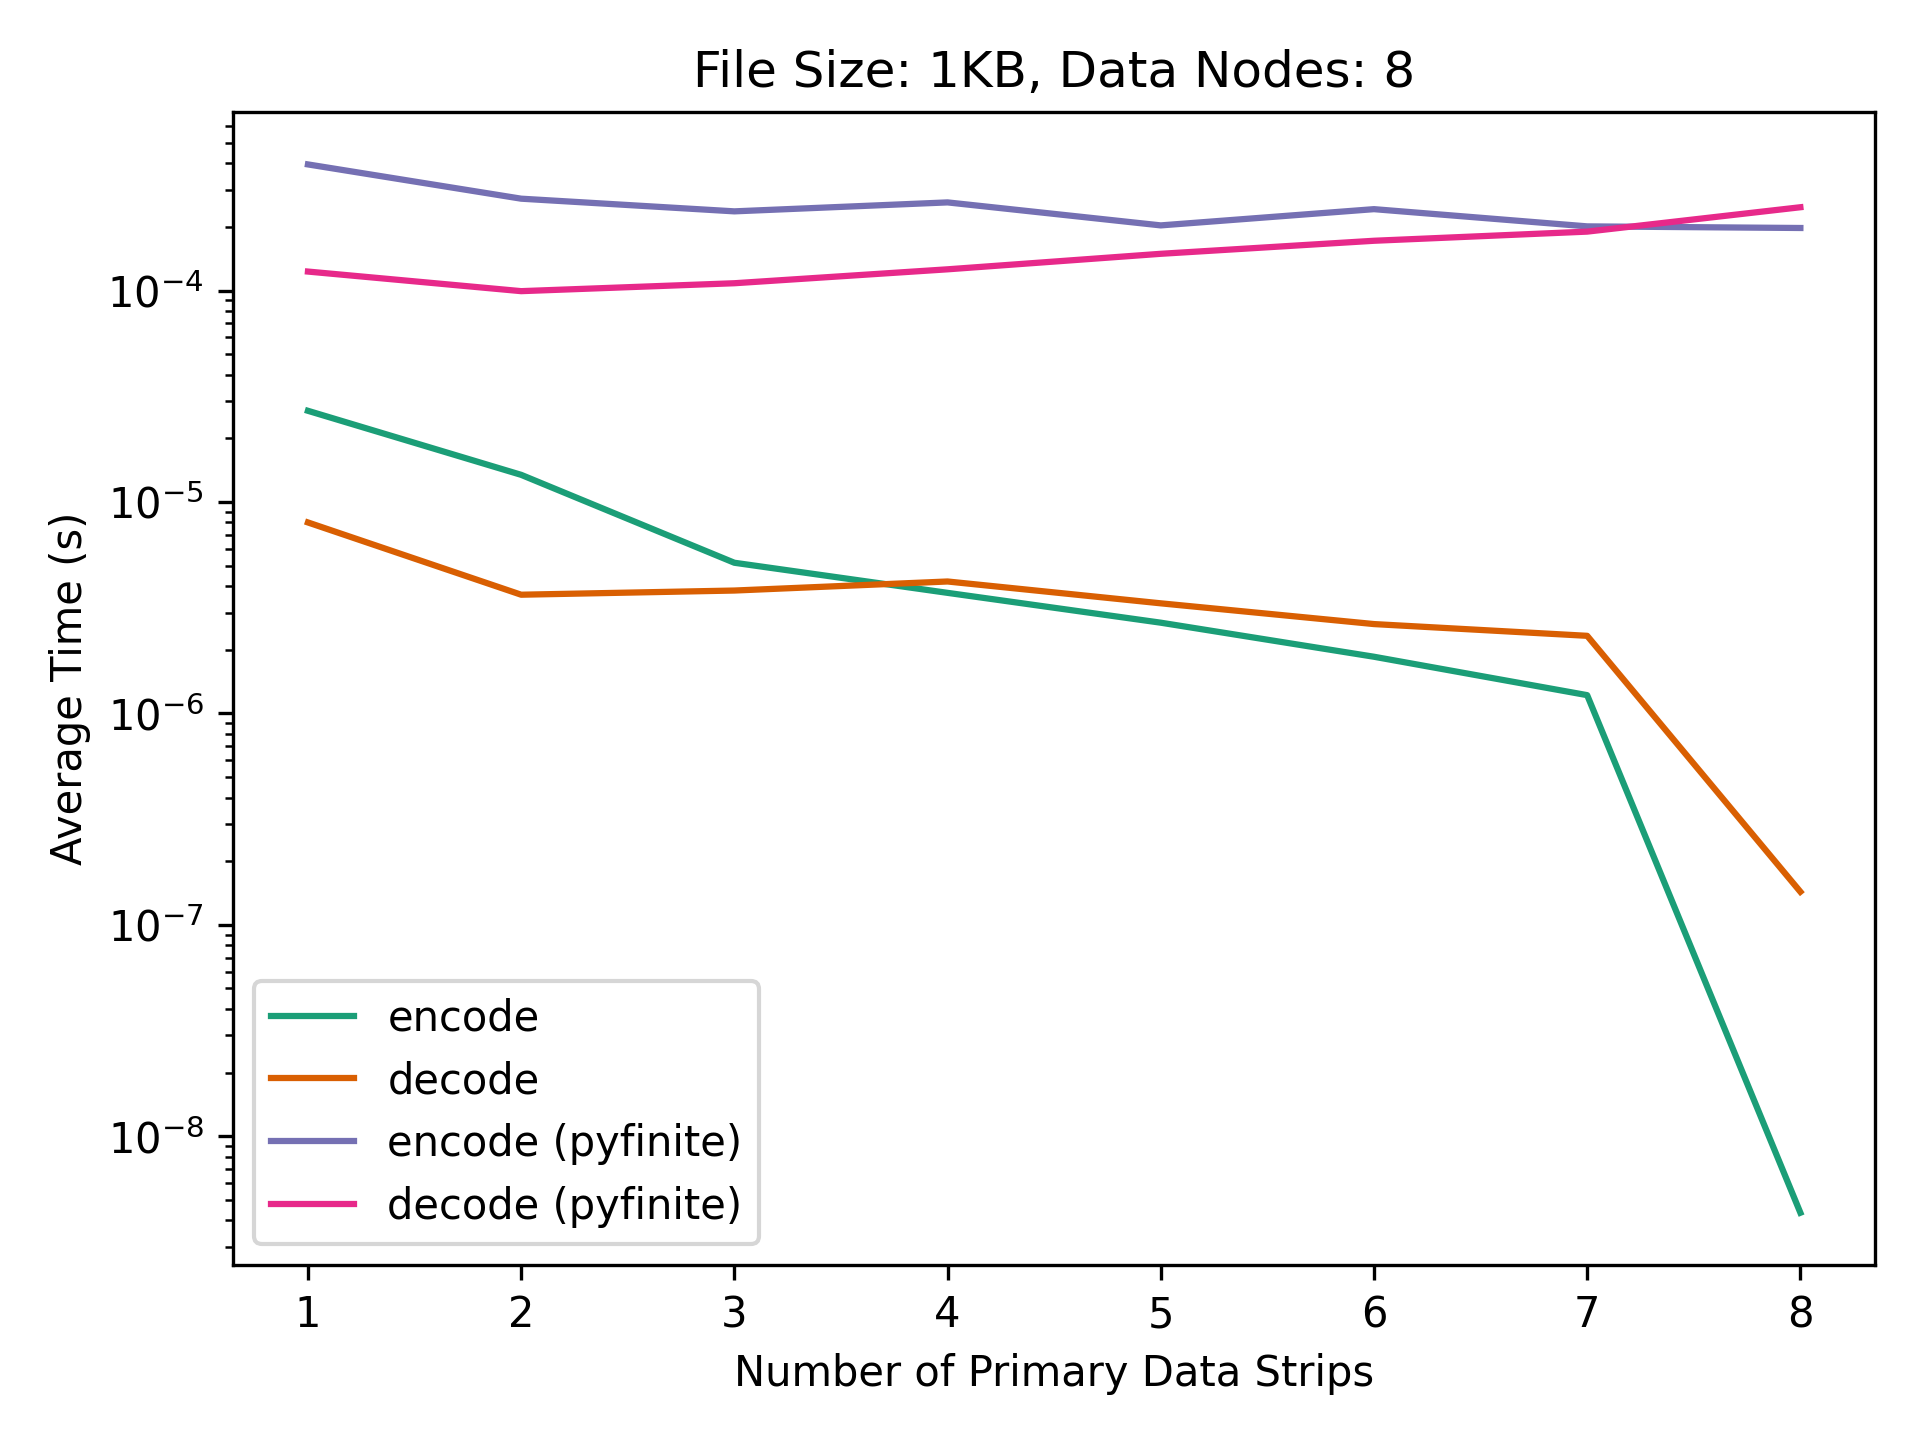
\includegraphics[width=0.8\columnwidth
]{images/encode-decode-size-1KB-n-8.png}
    \caption{1KB file with 8 data nodes.}
    \label{fig:encode-decode-1KB-8}
\end{figure}

\begin{figure}[htbp]
    \centering
    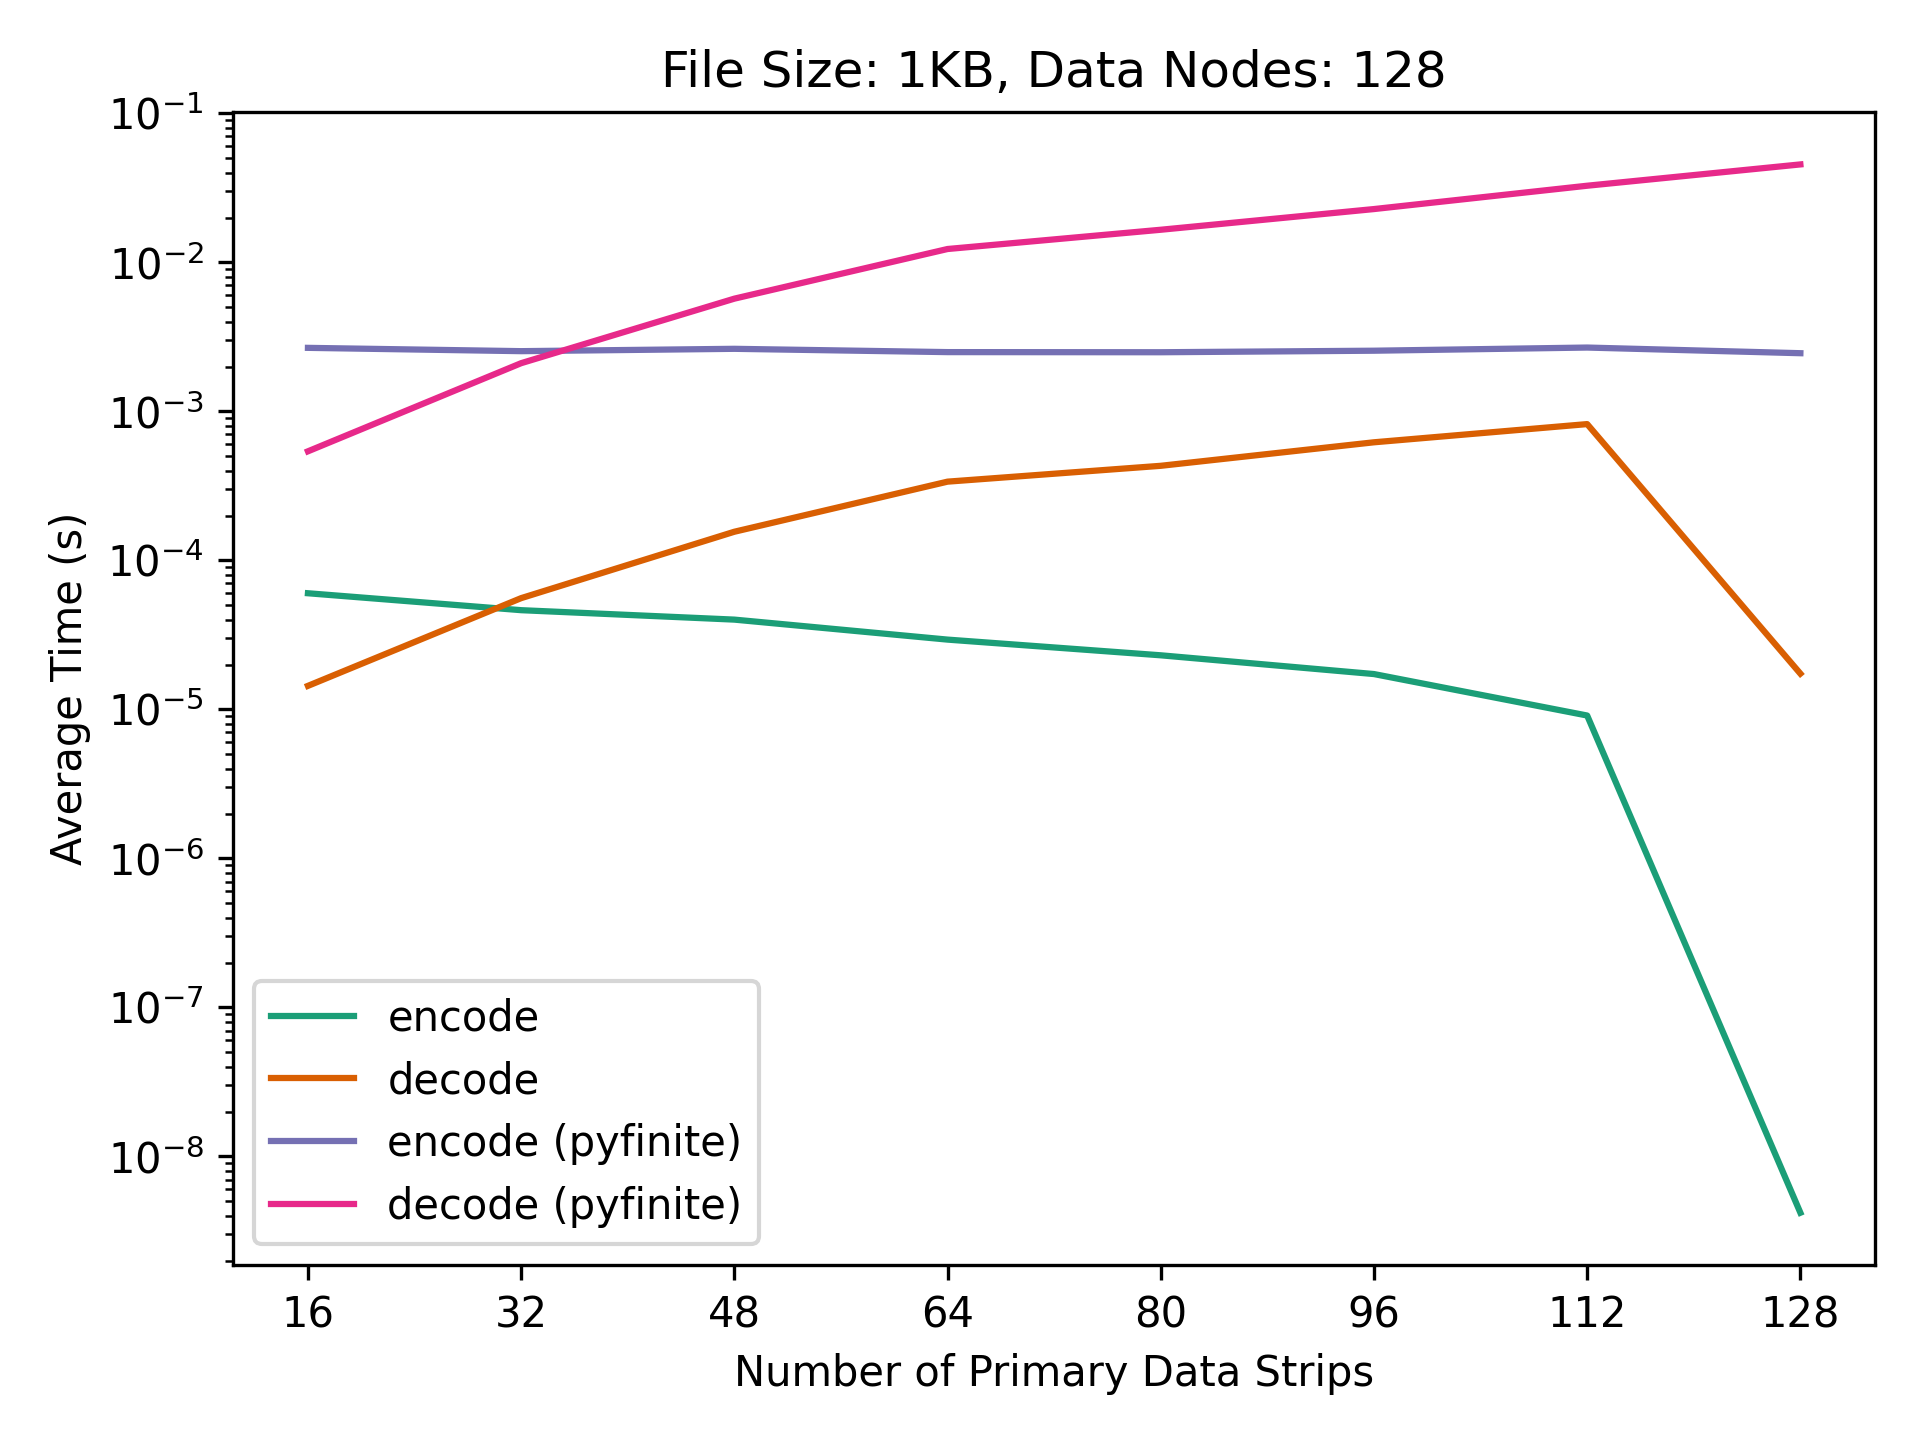
\includegraphics[width=0.8\columnwidth
]{images/encode-decode-size-1KB-n-128.png}
    \caption{1KB file with 128 data nodes.}
    \label{fig:encode-decode-1KB-128}
\end{figure}

\begin{figure}[htbp]
    \centering
    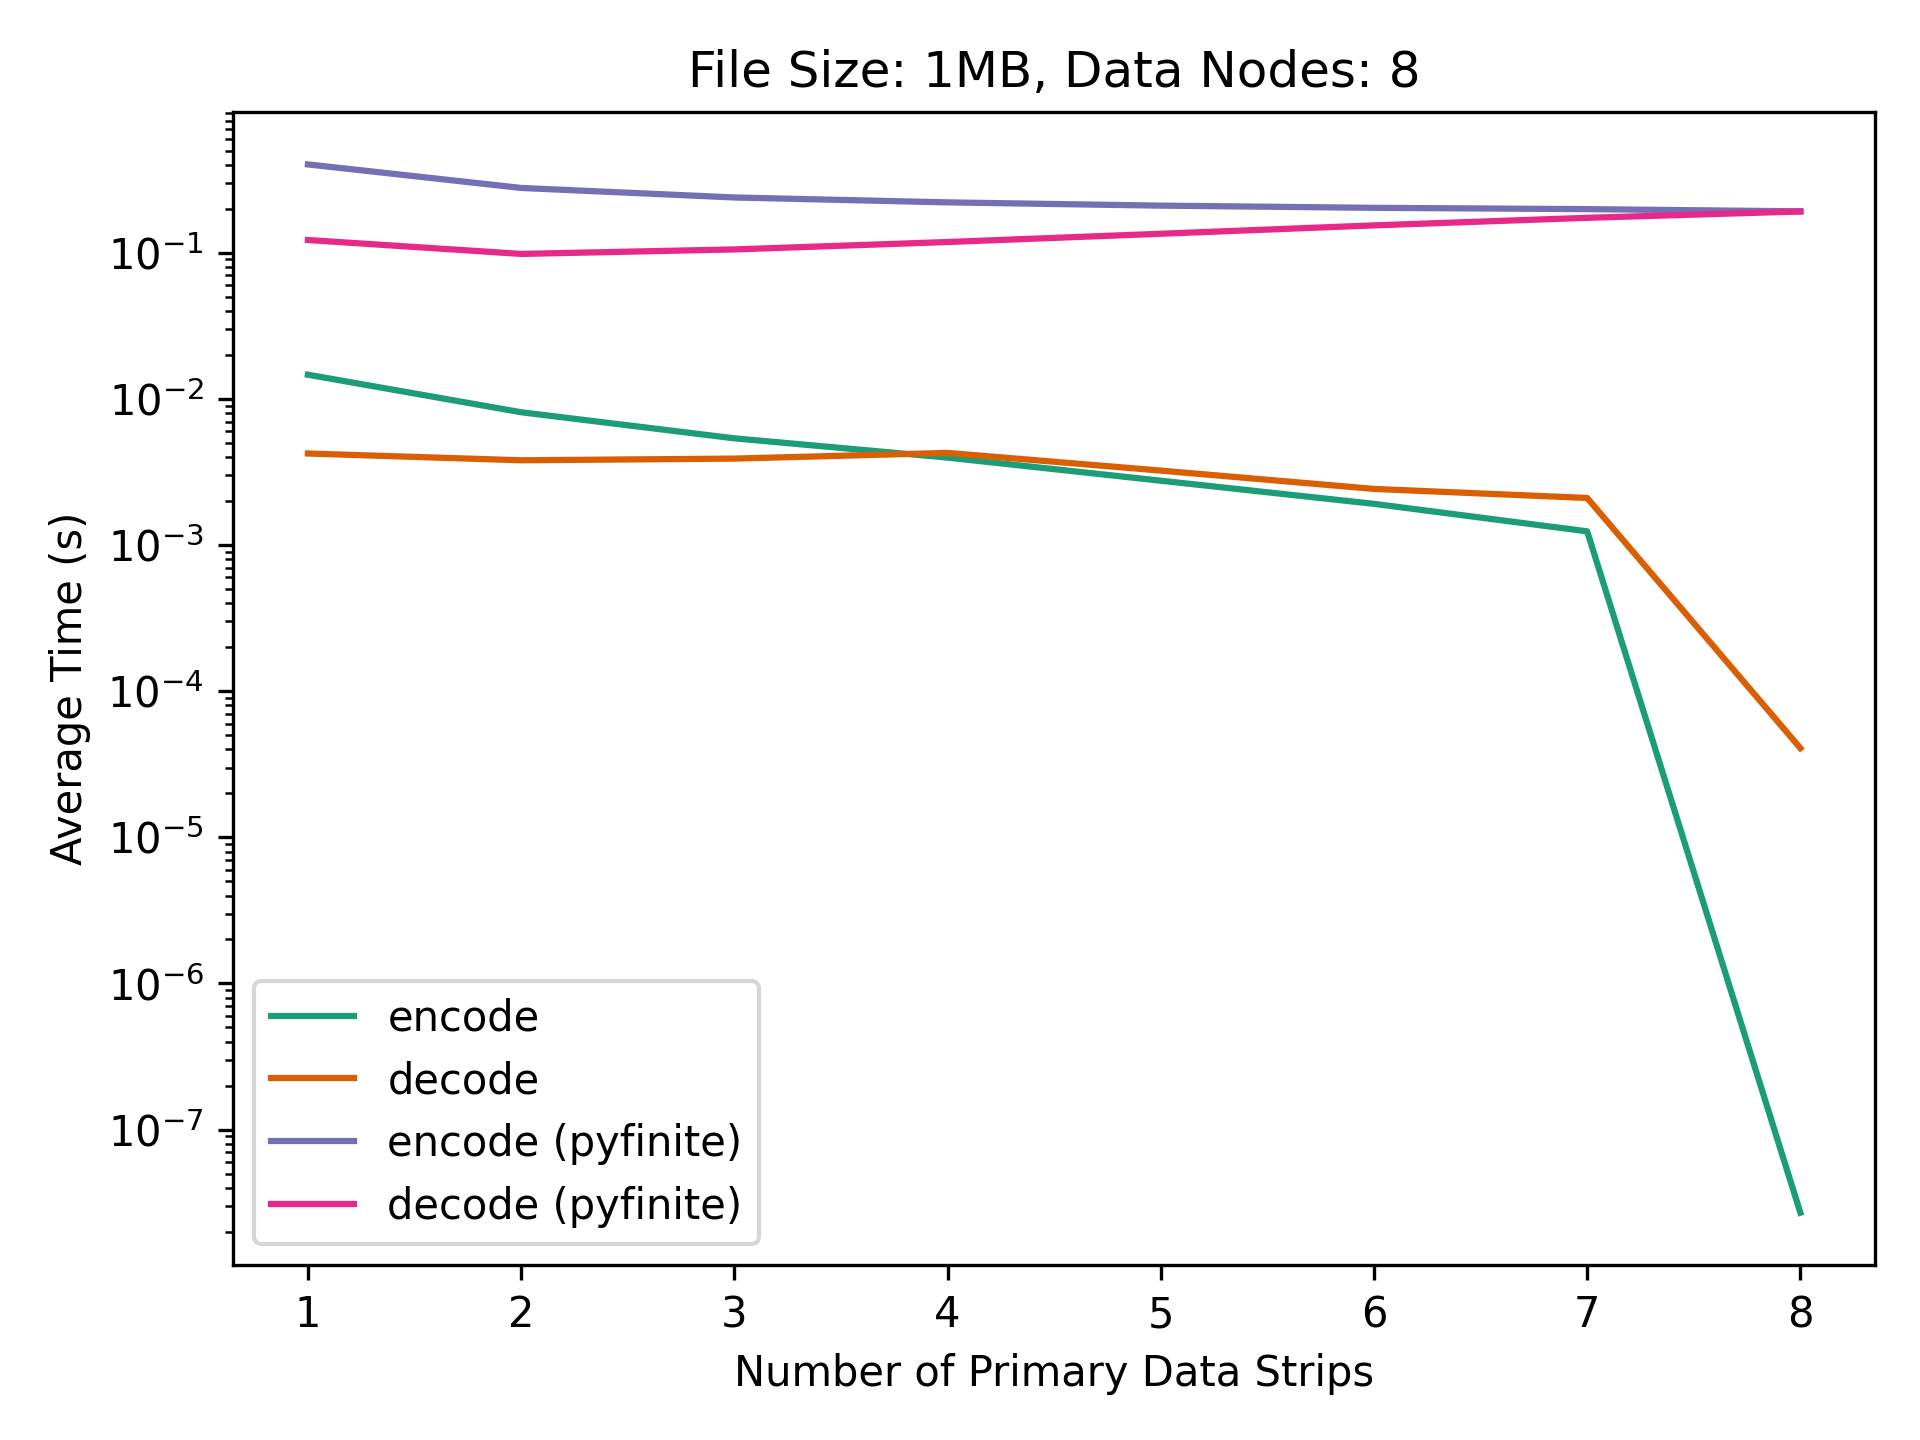
\includegraphics[width=0.8\columnwidth
]{images/encode-decode-size-1MB-n-8.png}
    \caption{1MB file with 8 data nodes.}
    \label{fig:encode-decode-1MB-8}
\end{figure}

\begin{figure}[htbp]
    \centering
    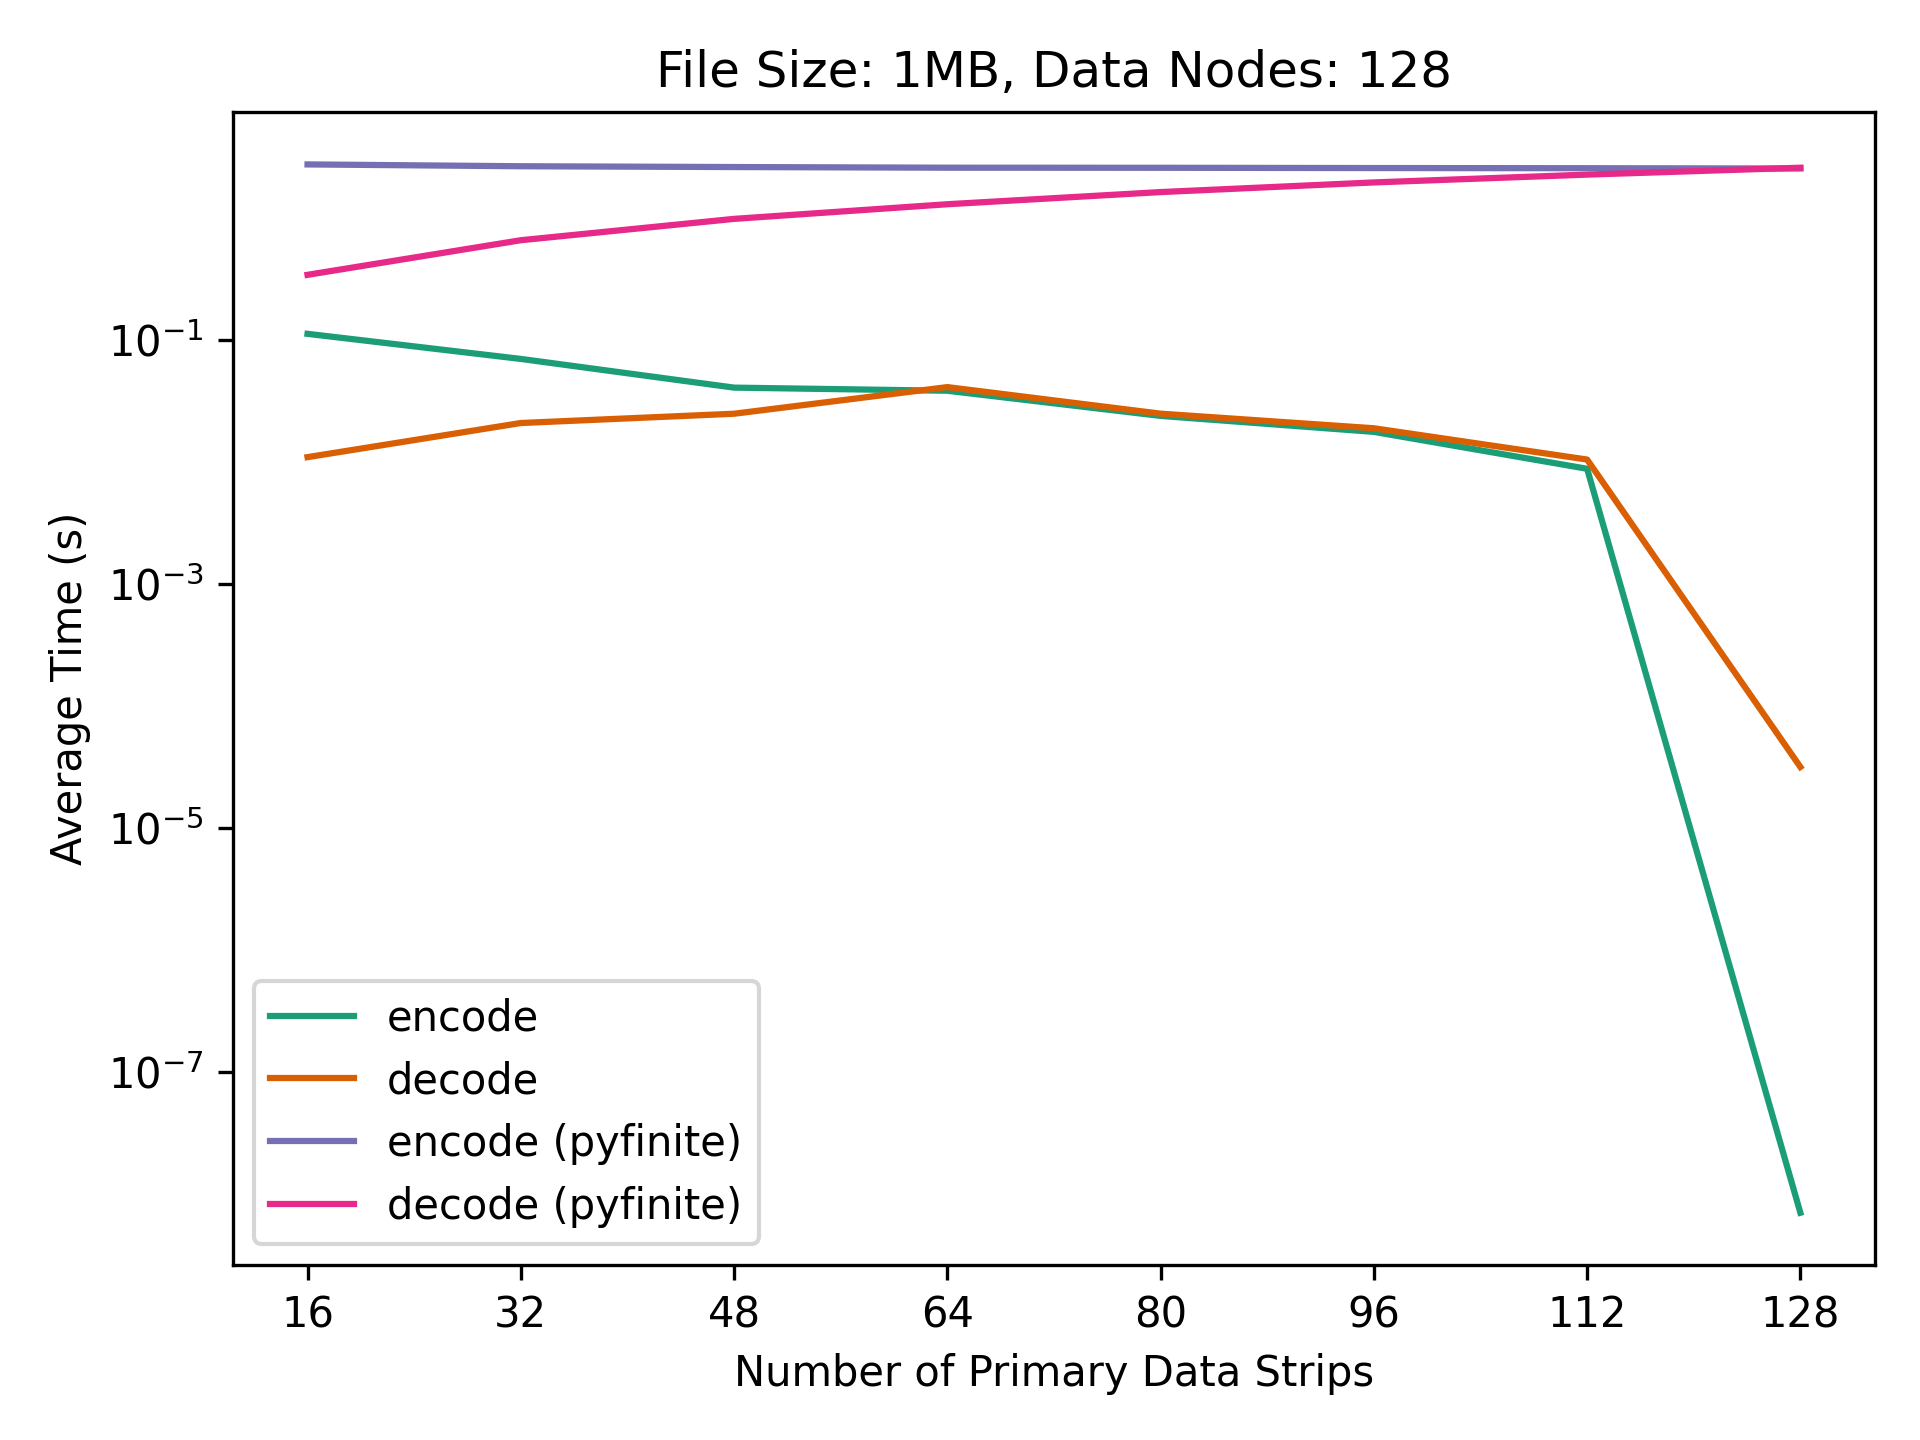
\includegraphics[width=0.8\columnwidth
]{images/encode-decode-size-1MB-n-128.png}
    \caption{1MB file with 128 data nodes.}
    \label{fig:encode-decode-1MB-128}
\end{figure}

We can find that for 1KB and 1MB files, the encoding and decoding time of our implementation is about 10-100 times faster than the \textit{pyfinite} library. Since the performance of the library is bad, we didn't test it for 1GB files because it will take too long time to encode and decode 1GB files.

\begin{figure}[htbp]
    \centering
    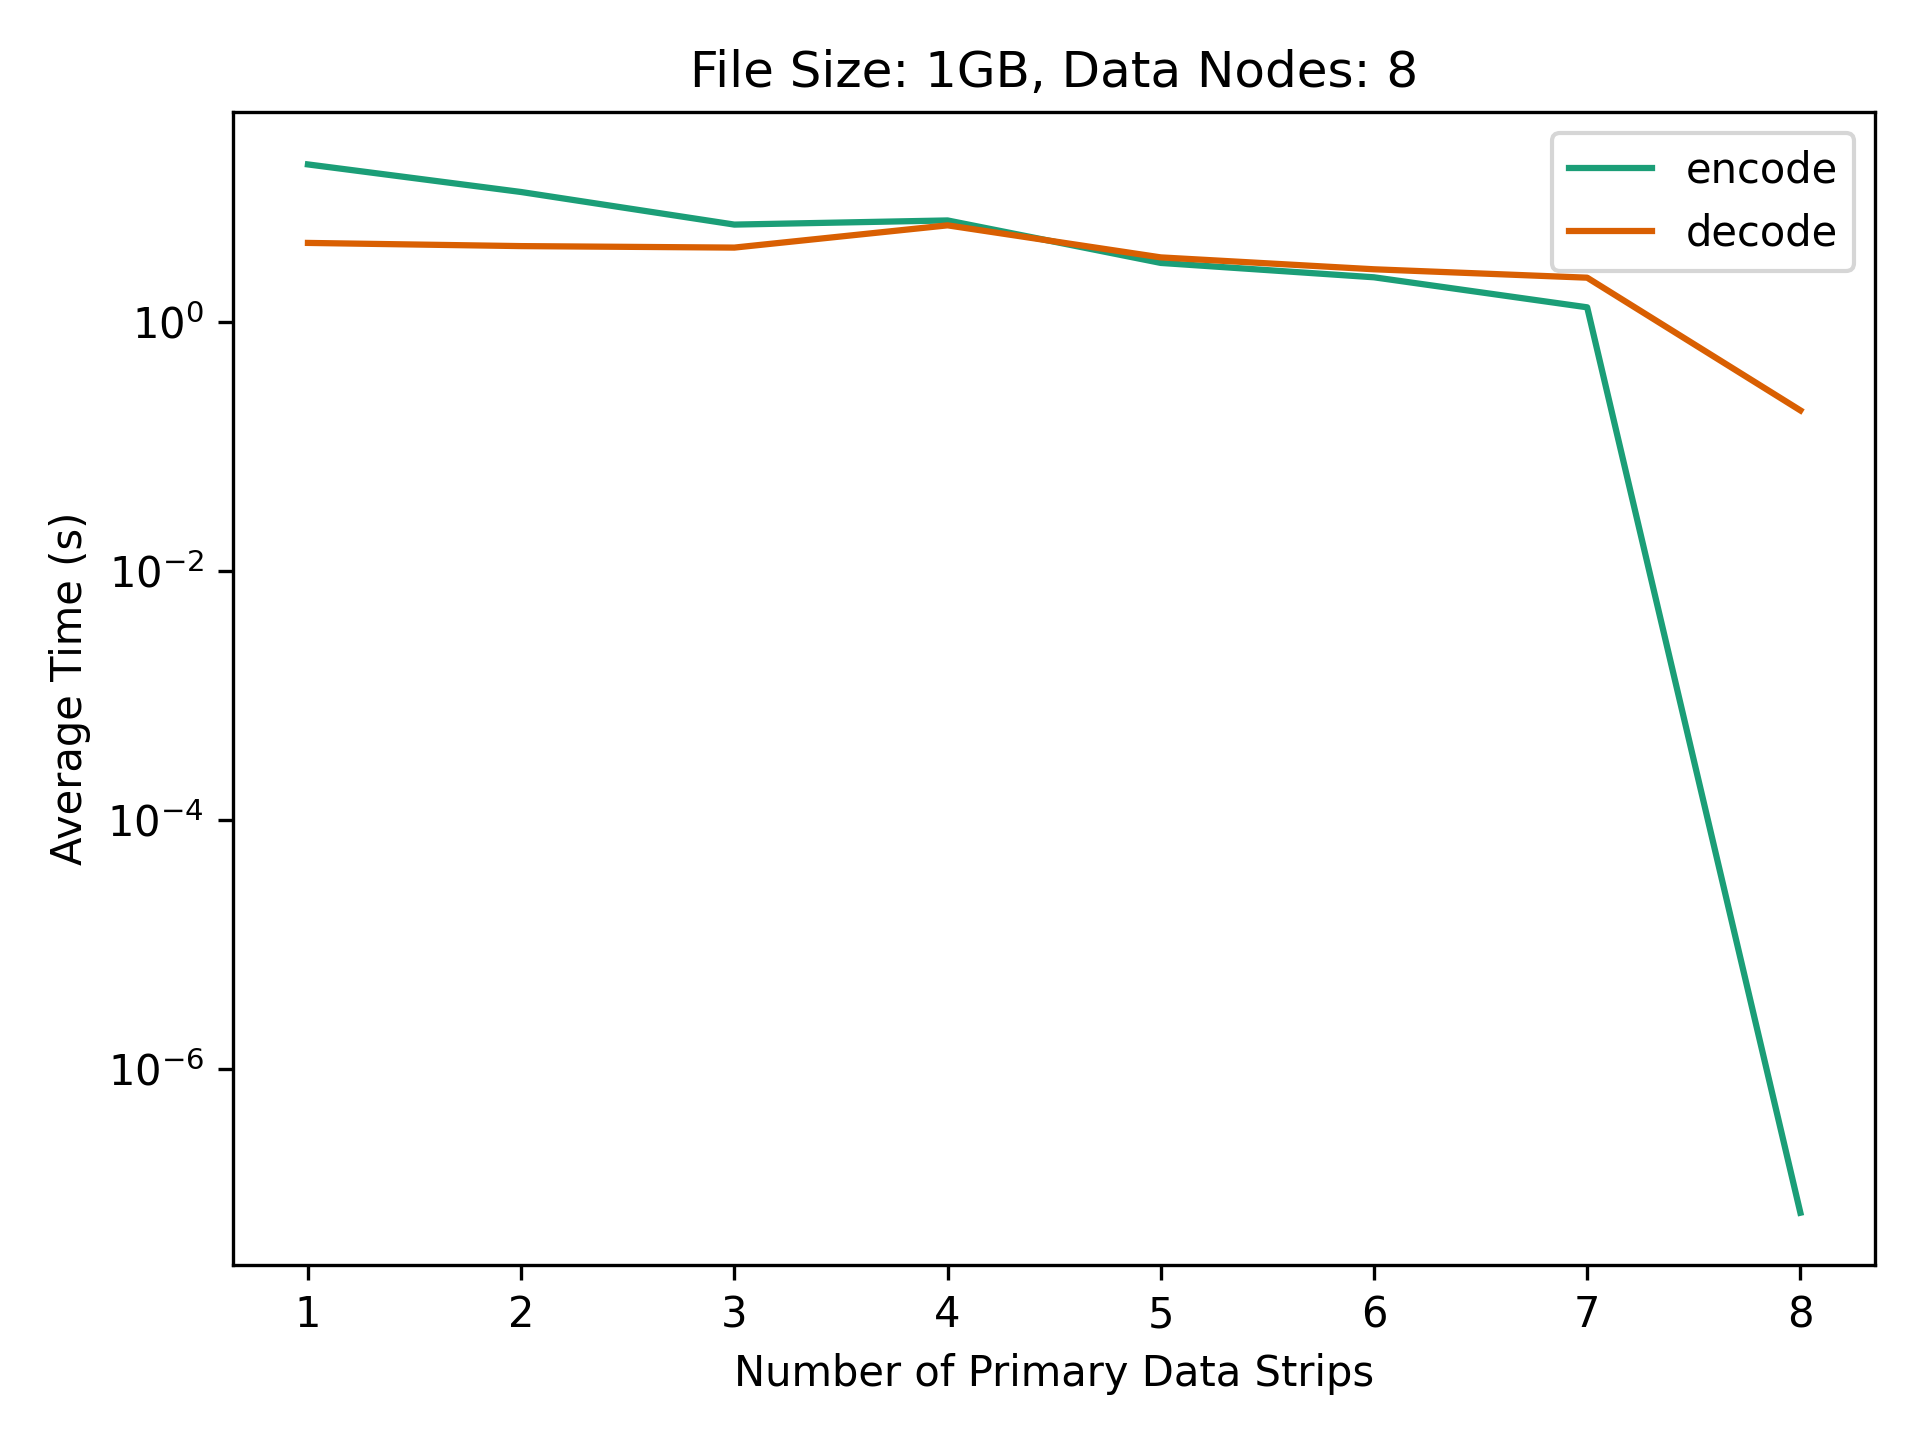
\includegraphics[width=0.8\columnwidth
]{images/encode-decode-size-1GB-n-8.png}
    \caption{1GB file with 8 data nodes.}
    \label{fig:encode-decode-1GB-8}
\end{figure}

\begin{figure}[htbp]
    \centering
    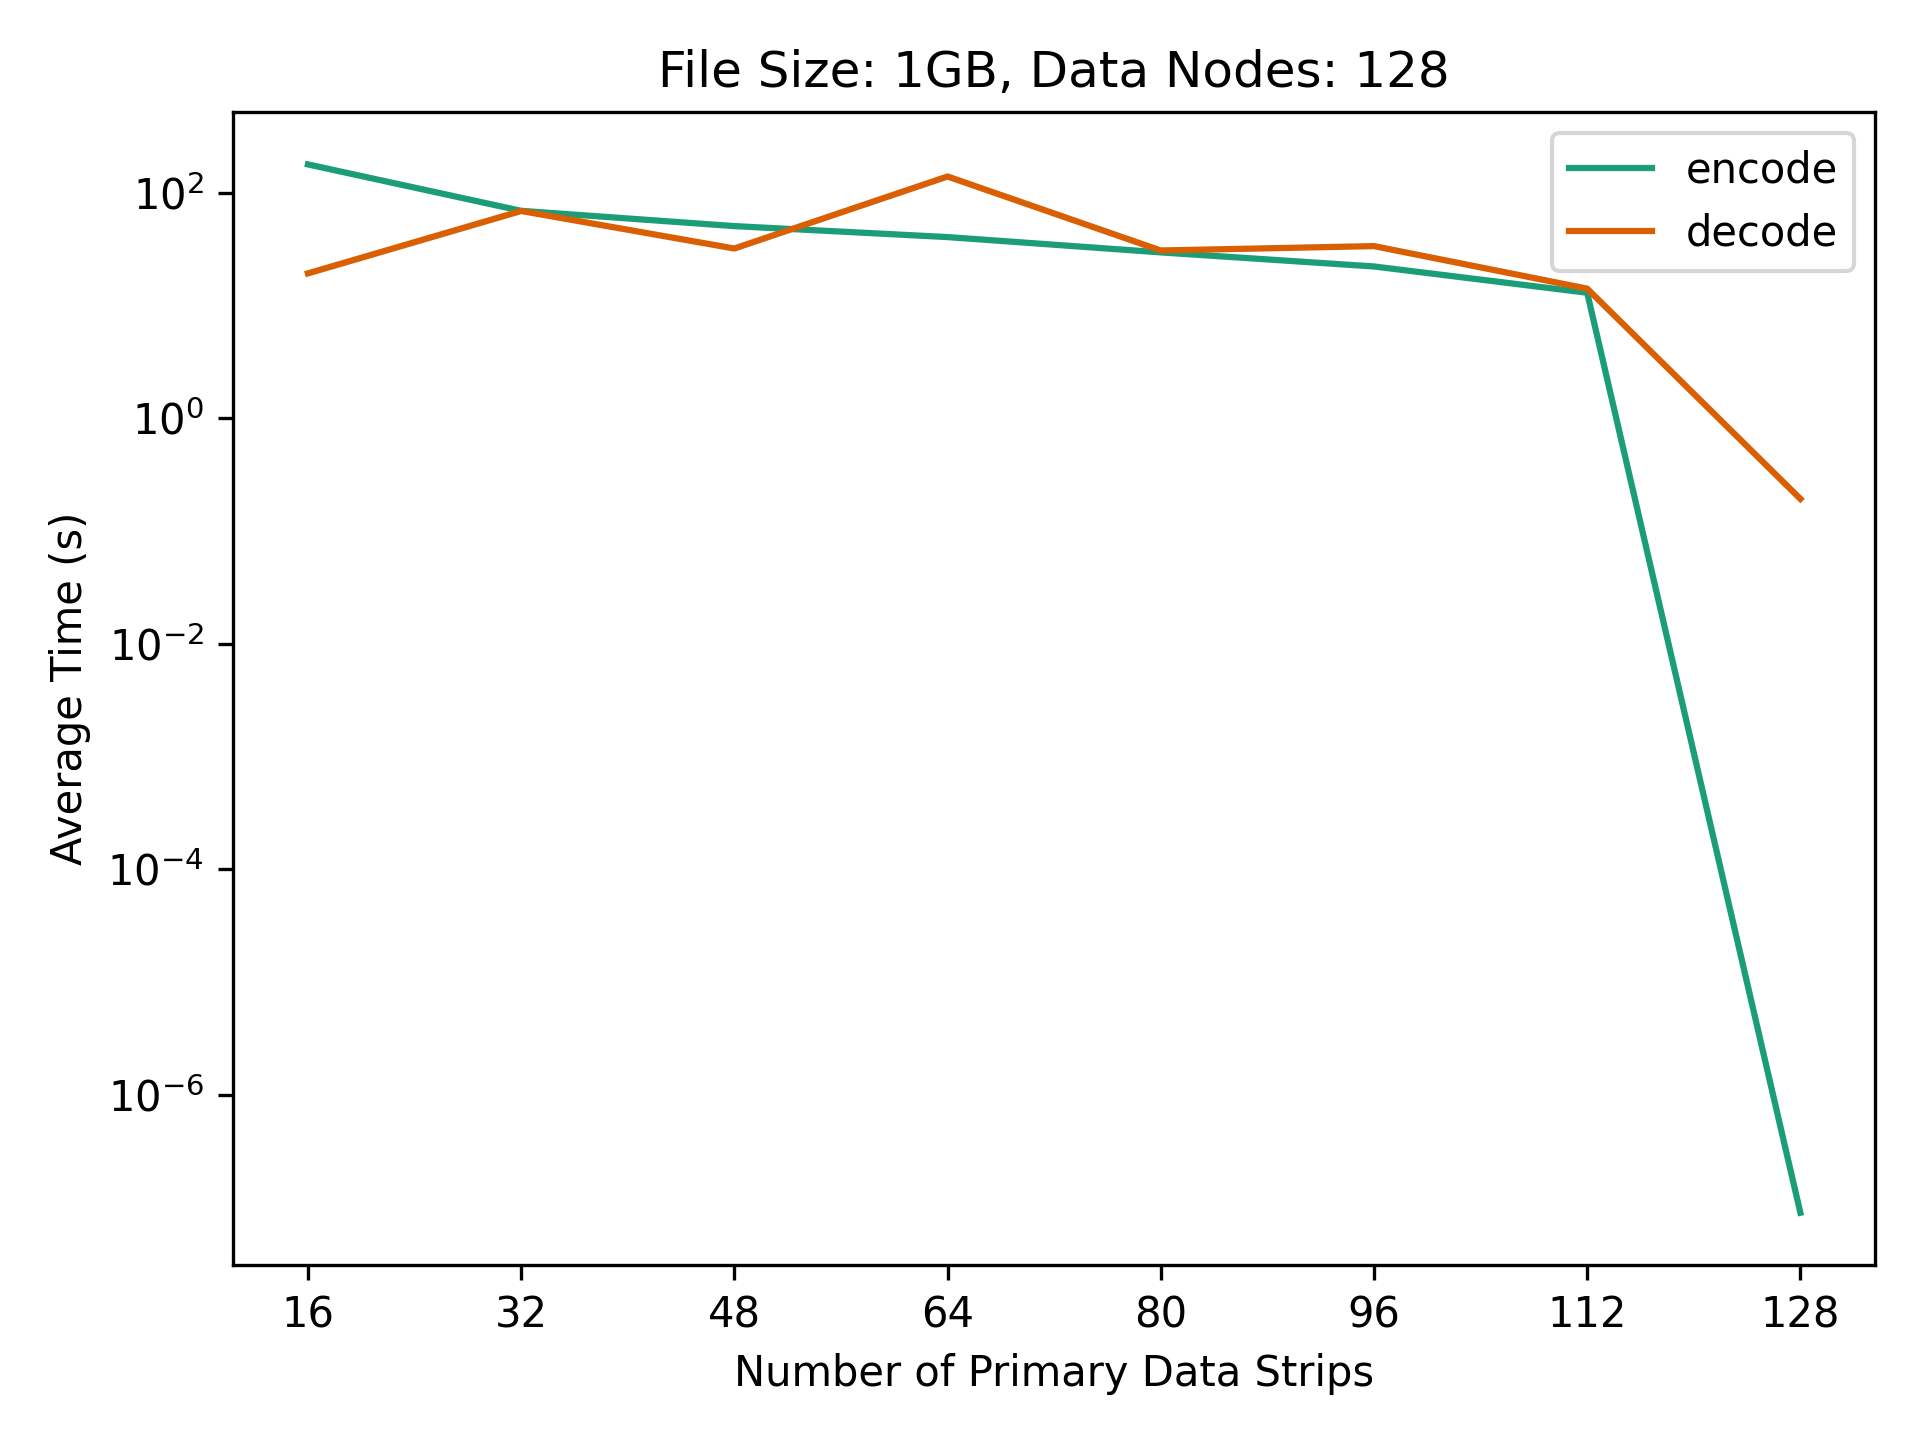
\includegraphics[width=0.8\columnwidth
]{images/encode-decode-size-1GB-n-128.png}
    \caption{1GB file with 128 data nodes.}
    \label{fig:encode-decode-1GB-128}
\end{figure}

\subsection{Performance of the P2P RAIN Network}

In this section, we use a standard 6+2 configuration to test the performance of our P2P RAIN network. We need to consider two different types of operations: the CPU-bound encode/decode operation and the IO-bound transmission operation. When a data object needs to be distributed over the network, we first encode it on one data node and then send it to all other data nodes; when a data objects needs to be read by a user on a data node, we first receive it from all other data nodes and then decode it on the used data node. So our experiment consists of all those four types of time, and the result is shown in Fig. \ref{fig:read-write}. 

\begin{figure}[htbp]
    \centering
    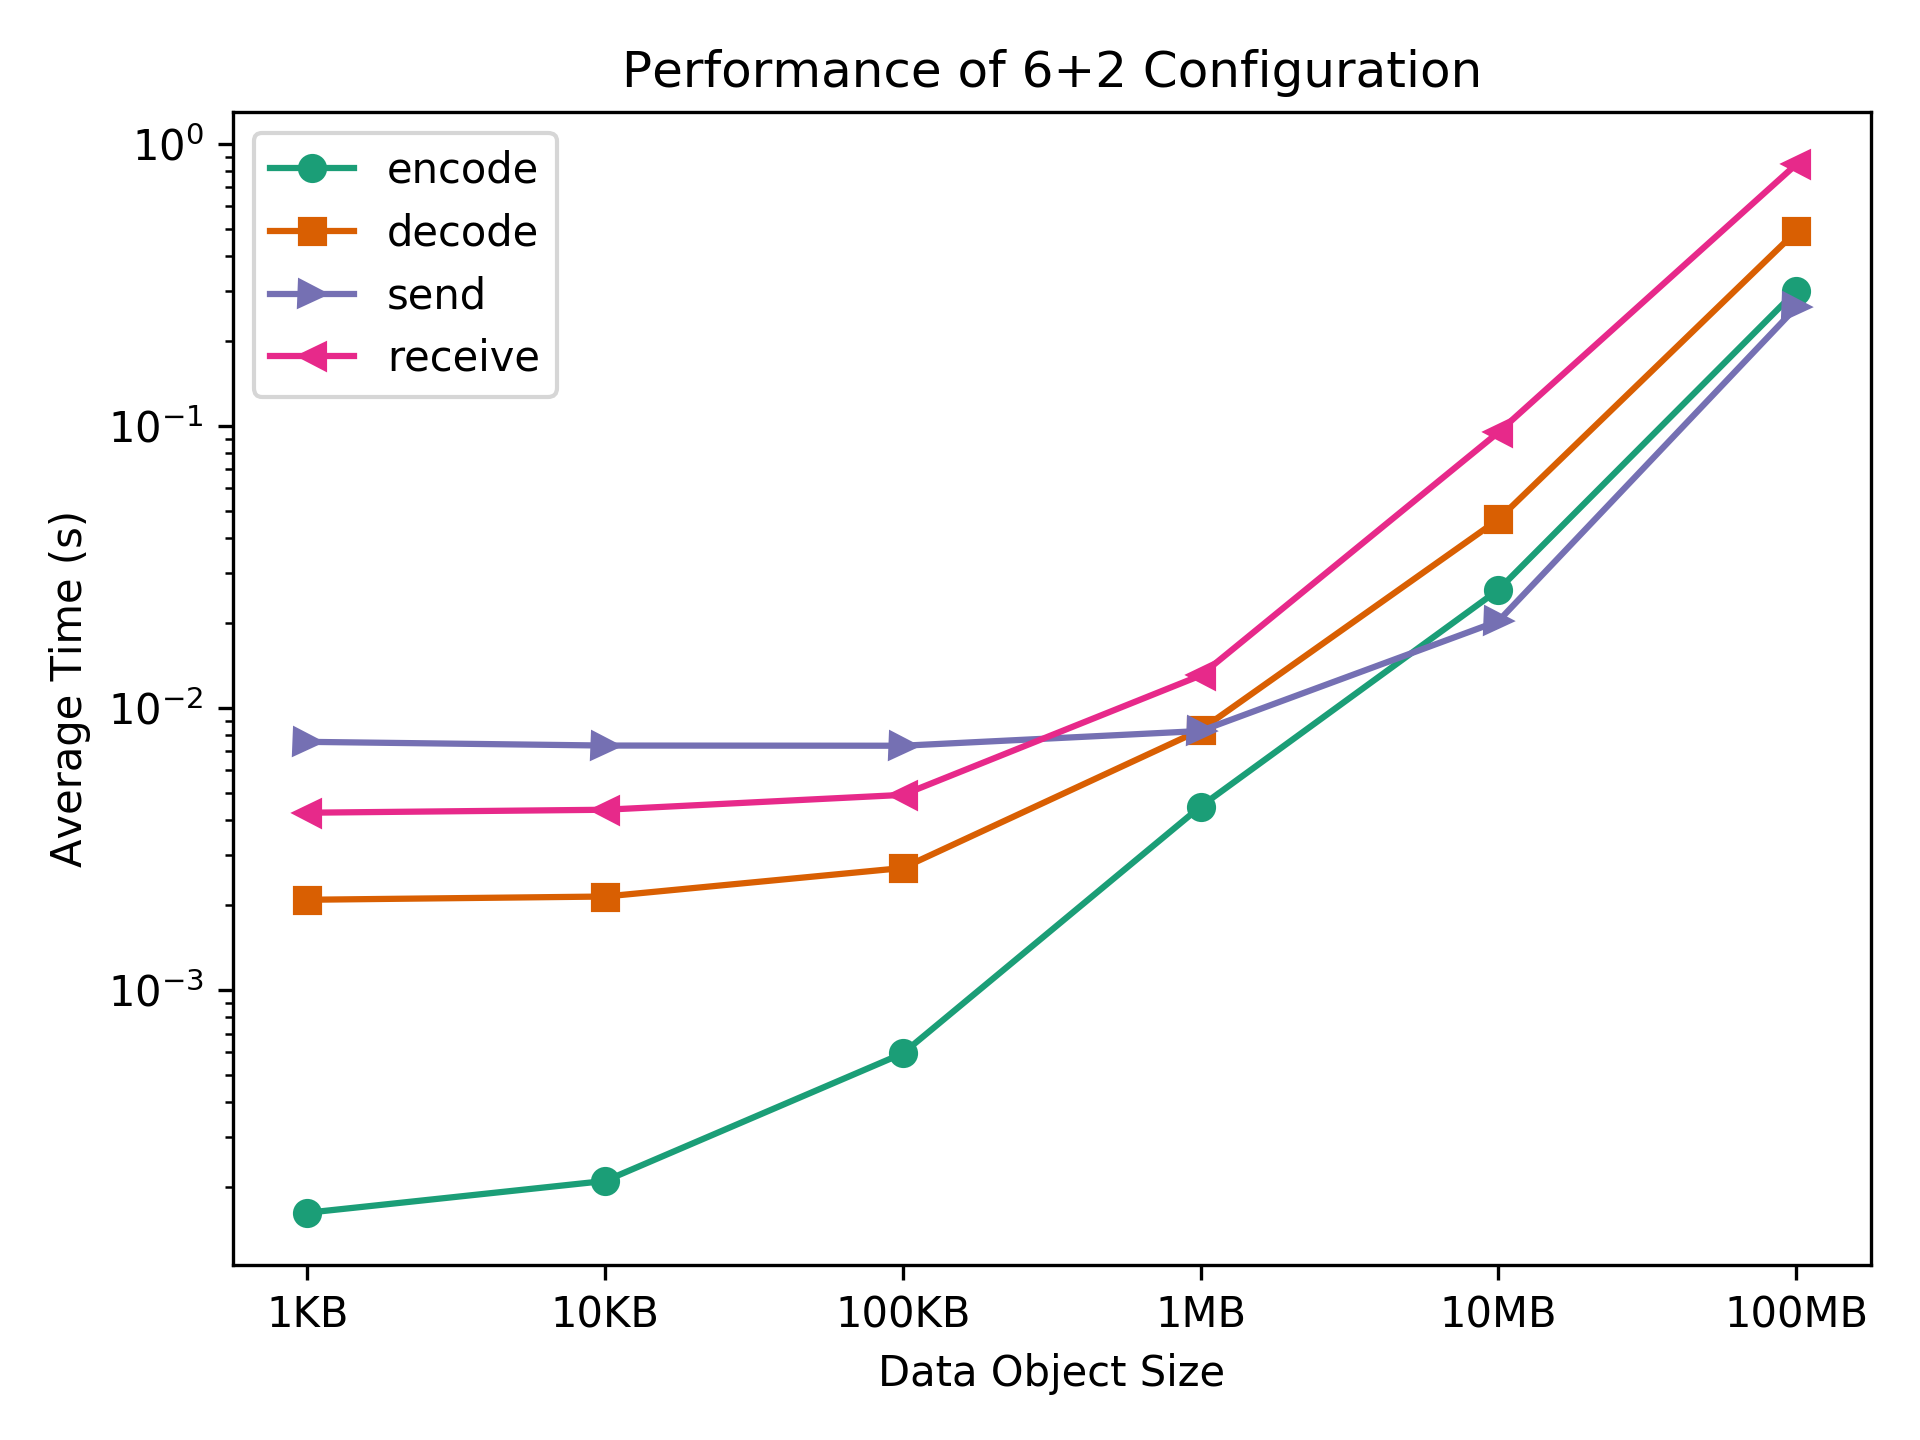
\includegraphics[width=0.8\columnwidth
]{images/read-write.png}
    \caption{Performance of the P2P RAIN Network.}
    \label{fig:read-write}
\end{figure}

We can observe from the graph that for small data objects (1KB to 100KB), the majority of time is used to transmit data over the network, and the time spent is very similar. This is because the time used to transfer a small data object is much more relevant to the network protocols used but the not actual size. The TCP protocol should include everything we need in a single datagram package in the transport layer for small files. However, for large files, the transmission time is linear to the data object size, which is also a reasonable result. 

We can also find that the performance of our encoding and decoding algorithm is enough for the P2P RAIN Network, because for large files, in the uploading file process, \textbf{encode} and \textit{send} takes similar time; in the downloading file process, \textbf{receive} even consumes more time than \textit{decode}, which becomes a bottleneck of the implementation. We discovered that the \textbf{receive} process may be further optimized to achieve a better performance in the system. 

Another finding is that for small data objects, decoding takes much longer time than encoding. This is because generating the inverse matrix takes constant time for different file sizes, but if the file size is too small, most time will be consumed to generate the inverse matrix, which leads to the effect shown in the figure.

\section{Conclusion}

In this project, we implemented a RAID-6 based distributed storage system to fulfill all the objectives in Section \ref{sec:intro}. We used C++ to implement a Reed-Solomon Code in file encoding and decoding and used Python to implement a peer-to-peer reliable array of independent nodes network to carry out communication between different data nodes. The experiment result shows that our system is robust and adaptive while retaining a reasonable time complexity.

\bibliographystyle{IEEEtran}
\bibliography{main}


\end{document}
